\subsection{Generalizations}

Thisundefinedsectionundefinedfocusesundefinedonundefinedmoreundefinedgeneralundefinedcases.undefinedInundefinedparticular,

\begin{enumerate}
\item \textbf{MultipleundefinedConstraint},undefinedi.e.,undefinedinundefinedtheundefinedcaseundefinedof

\begin{equation}
J=\int f(x,y_1,y_2,...,y_n,\dot y_1, \dot y_2,...,\dot y_n, \ddot y_1,...)
\end{equation}


\item \textbf{VariableundefinedEndpoints}
Inundefinedpreviousundefinedcases,undefinedweundefinedusedundefinedtheundefinedkeyundefinedassumptionundefinedthat:
\end{enumerate}

\begin{mystadmonition}{mystAmber}{FixedundefinedEndpointundefinedAssumption}Theundefinedperturbationundefined$\delta y$undefinedisundefined0undefinedatundefinedendpoints,undefinedhenceundefinedallundefinedboundary/surfaceundefinedtermsundefinedarisingundefinedfromundefinedintegartionundefinedbyundefinedpartsundefinedmayundefinedbeundefinedignored.

\end{mystadmonition}
Weundefinednowundefinedrelaxundefinedthisundefinedassumptionundefinedbutundefinedratherundefinedworkundefinedoutundefinedboundaryundefinedconditionsundefinedbasedundefinedonundefinedtheundefinedstationaryundefinedconditionundefinedwithundefinedvariableundefinedendpoints.undefinedThisundefinedassumptionundefinedcanundefinedinundefinedturnundefinedbeundefinedappliedundefinedtoundefinedtheundefinedresultingundefineddifferentialundefinedequations.

\begin{enumerate}[resume]
\item \textbf{ConstrainedundefinedOptimization}undefinedOften,undefinedtheundefinedminimizationundefinedofundefinedtheundefinedactionundefinedisundefinedsubjectedundefinedtoundefinedphyscialundefinedconstraint.undefinedForundefinedinstance,undefinedinundefinedtheundefinedfamousundefined\textit{catenaryundefinedproblem},undefinedweundefinedneedundefinedtoundefinedfixundefinedtheundefinedlengthundefinedofundefinedtheundefinedhangingundefinedchain.
\end{enumerate}

\subsubsection{MultipleundefinedConstraint}

\subsubsection{VariableundefinedEndpoints}

\subsubsection{ConstraintundefinedOptimization}

\subsubsection{Exercises}

\paragraph{ElasticundefinedRods}

\begin{mystadmonition}{mystAmber}{ElasticundefinedRods}\begin{itemize}
\item Theundefined\textbf{elasticundefinedenergyundefinedperundefinedunitundefinedlength}undefinedofundefinedaundefinedbentundefinedsteelundefinedrodundefinedisundefinedgivenundefinedbyundefined

\begin{equation}
\frac{1}{2}\frac{YI}{R^2}
\end{equation}


HereundefinedYundefinedisundefinedtheundefined\textit{Young'sundefinedmodulus}undefinedofundefinedtheundefinedsteelundefinedandundefined$I$undefinedisundefinedtheundefinedmomentundefinedofundefinedinertiaundefinedofundefinedtheundefinedrod'sundefinedcrossundefinedsectionundefinedaboutundefinedanundefinedaxisundefinedthroughundefineditsundefinedcentroidundefinedandundefinedperpendicularundefinedtoundefinedtheundefinedplaneundefinedinundefinedwhichundefinedtheundefinedrodundefinedisundefinedbent.
\end{itemize}

\begin{itemize}
\item Letundefinedusundefinedassumeundefinedtheundefinedrodundefinedisundefinedonlyundefinedslightlyundefinedbentundefinedintoundefinedtheundefinedyzundefinedplaneundefinedandundefinedliesundefinedcloseundefinedtoundefinedtheundefinedzundefinedaxis.undefinedRundefinedisundefinedtheundefinedradiusundefinedofundefinedcurvatureundefineddueundefinedtoundefinedtheundefinedbending,undefinedrelatedundefinedtoundefinedtheundefinedcurvatureundefinedby

\begin{equation}
\frac{1}{R}=\kappa = |T_z|
\end{equation}


whereundefined$T$undefinedisundefinedtheundefinedunitundefinedtangentundefinedvectorundefinedtoundefinedtheundefinedrod.
\end{itemize}

\subparagraph{Problemundefined0}

Showundefinedthatundefinedtheundefinedelasticundefinedenergyundefinedcanundefinedbeundefinedapproximatedundefinedby:
\begin{equation}
\boxed{U[y]=\int_0^L \frac12 \left\{ \frac{1}{2} YI(y'')^2 \right\}dz}
\end{equation}

\subparagraph{Problemundefined1}

Theundefinedrodundefinedisundefinedusedundefinedasundefinedaundefinedcolumnundefinedwhichundefinedsupportsundefinedaundefinedcompressiveundefinedloadundefined$Mg$undefineddirectedundefinedalongundefinedtheundefinedzundefinedaxisundefined(whichundefinedisundefinedvertical).undefinedShowundefinedthatundefined:

\textbf{(a)}undefinedwhenundefinedtheundefinedrodundefinedbucklesundefinedslightlyundefined(i.e.undefinedbendsundefinedwithundefinedbothundefinedendsundefinedremainingundefinedonundefinedtheundefinedzundefinedaxis)undefinedthe
totalundefinedenergy,undefinedincludingundefinedtheundefinedgravitationalundefinedpotentialundefinedenergyundefinedofundefinedtheundefinedloadingundefinedmassundefinedM,undefinedcanundefinedbe
approximatedundefinedby
\begin{equation}
\boxed{U[y]=\int_0^L \left\{ \frac{YL}{2} (y'')^2 - \frac{Mg}{2}(y')^2\right\}dz}
\end{equation}

\textbf{(b)}undefinedByundefinedconsideringundefineddeformationsundefinedofundefinedtheundefinedform
\begin{equation}
y(z)=\sum_{n=1}^{\infty} a_n\sin(\frac{n\pi z}{L})
\end{equation}
showundefinedthatundefinedtheundefinedcolumnundefinedisundefinedunstableundefinedtoundefinedbucklingundefinedandundefinedcollapseundefinedonce
\begin{equation}
Mg \geq \frac{\pi^2}{L^2}YI
\end{equation}

\subparagraph{}

\end{mystadmonition}
\begin{figure}[!htbp]
\centering
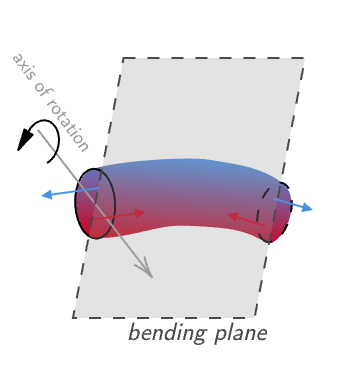
\includegraphics[width=0.375\linewidth]{files/bending_beam-3f593e81e849dc20a7466f2be18f704f.png}
\caption*{Bendingundefinedbeamundefinedandundefinedtheundefinedaxisundefinedofundefinedrotationundefinedassociatedundefinedwithundefinedtheundefinedmomentundefinedofundefinedundefinedinertiaundefined$I$}
\end{figure}

\begin{mystadmonition}{mystGreen}{SolutionundefinedtoundefinedProblemundefined0}Weundefinedneedundefinedaundefinedlittleundefinedlemma(orundefinedrecallundefinedfromundefinedCalculusundefinedI):
\begin{equation}
\kappa = \frac{y''}{(1+y'^2)^{3/2}}
\end{equation}

Forundefinedsmallundefinedperturbationundefined$|y'|\ll 1$undefinedhenceundefined$(1+y'^2)^{\frac32} \approx 1$undefinedhence
$\kappa = \frac{1}{R}=(y'')$.undefinedSquaringundefineditundefinedweundefinedhaveundefined:
\begin{equation}
\frac{1}{R^2}=(y'')^2
\end{equation}
Hence:
\begin{equation}
dU=\frac12 YI (y'')^2 dz
\end{equation}
Integratingundefinedgetundefinedusundefinedtheundefineddesiredundefinedresult.

\begin{mystthmproof}{Proofundefinedofundefinedlemma}{proof-generalizations-1}Ifundefinedweundefinedimagineundefinedweundefinedtraverseundefinedalongundefinedaundefinedcurveundefined$\Gamma$,undefinedtheundefinedaccelearationundefinedwouldundefinedbe:
\begin{equation}
\begin{aligned}
r''(z) &= \frac{d}{dz}\left(\frac{dr}{dz}\right) \\
&=  \frac{d}{dz}\left(\frac{ds}{dz}T\right)  \\
&= \frac{d^2s}{dz^2}T + \frac{ds}{dz}\frac{dT}{dz}
\end{aligned}
\end{equation}
Noteundefinedthatundefined
\begin{equation}
\left\langle T, \frac{dT}{dz}\right\rangle=0
\end{equation}
sinceundefined$|T|=1$.undefinedThereforeundefined$r''(z)$undefinedcanundefinedbeundefineddecomposedundefinedtoundefinedaundefinedtangentialundefinedcomponentundefined$\frac{d^2s}{dz^2}T$undefinedandundefinedaundefinedcentrepetalundefinedcomponentundefined$\frac{ds}{dz}\frac{dT}{dz}$.
Also,undefined$\frac{dT}{dz}$undefinedisundefinedco-linearundefinedwithundefinedourundefinedquanittyundefinedofundefinedinterest
\begin{equation}
\frac{dT}{dz}=\frac{dT}{ds}\frac{ds}{dz}
\end{equation}
Therefore:
\begin{equation}
\boxed{r''(z)= \frac{d^2s}{dz^2}T + \left(\frac{ds}{dz}\right)^2 \frac{dT}{ds}}
\end{equation}
Weundefinedcanundefinedisolateundefinedtheundefinedcentrepetalundefinedcomponentundefinedbyundefinedapplyundefinedaundefinedcrossundefinedproduct:
\begin{equation}
\begin{aligned}
T\times r''(z) &= T \times \left(\frac{ds}{dz}\right)^2\frac{dT}{dz}
\end{aligned}
\end{equation}
Nowundefined:

\begin{enumerate}
\item (LHS)undefined$T=(1,0,y')/ds$,undefinedhenceundefined$r''(z) = (0,0,y'')$.undefinedHenceundefinedtheundefinedcrossundefinedproductundefinedis:

\begin{equation}
\frac{1}{\sqrt{1+y'^2}} (1,0,y')^T \times (0,0,y'')  = \frac{1}{\sqrt{1+y'^2}}(0,y'',0)^T
\end{equation}


\item (RHS)undefinedSinceundefined$T, \frac{dT}{dz}$undefinedareundefinedorthogonalundefinedtoundefinedeachundefinedotherundefinedandundefinedbothundefinedlieundefinedinundefinedtheundefinedx-zundefinedplane,undefinedweundefinedhave:

\begin{equation}
T \times \left(\frac{ds}{dz}\right)^2\frac{dT}{dz} =  \left(\frac{ds}{dz}\right)^2 \textcolor{brown}{\left|\frac{dT}{dz}\right|} (0,1,0)^T
\end{equation}
\end{enumerate}

Nowundefinedcombiningundefinedtheundefinedaboveundefinedtwoundefinedequations,undefinedweundefinedget:
\begin{equation}
\frac{y''}{\sqrt{1+y'^2}}=\left(\frac{ds}{dz}\right)^2  \left|\frac{dT}{dz}\right|
\end{equation}
Asundefineddesired.

\end{mystthmproof}
\end{mystadmonition}
\begin{mystadmonition}{mystGreen}{SolutionundefinedtoundefinedProblemundefined1}(a)undefinedConsiderundefinedtheundefinedschemeticundefinedabove.undefinedSupposeundefined$y=0$undefinedforundefined$z\in (L -dL,L)$,undefinedthen
\begin{equation}
\begin{aligned}
L+dL&=\int_0^L \sqrt{1+y'^2}dz \\ 
&\approx \int_0^L 1 + \frac{1}{2}y'^2dz\\
&= L + \int_0^L \frac{1}{2}y'^2dz
\end{aligned}
\end{equation}
Henceundefined$dL=\int_0^L \frac{1}{2}y'^2$.undefinedIfundefinedweundefinedconsiderundefinedtheundefinedgravitationalundefinedpotentialundefinedenergyundefinedtoundefinedbeundefined0undefinedatundefined$h=L$,undefinedthenundefinedtheundefinedgravitationalundefinedpotentialundefinedenergyundefinedbecomes:
\begin{equation}
-\int_0^L \frac{1}{2}y'^2dz
\end{equation}
theundefinednegativeundefinedsignundefinedisundefinedthereundefinedtoundefinedaccountundefinedforundefinedcompression.undefinedCombiningundefinedwithundefinedtheundefinedresultundefinedfromundefinedproblemundefined0undefinedweundefinedgetundefinedasundefineddesired.

(b)undefinedTheundefinedEuler-Lagrangeundefinedequationundefinedforundefinedtheundefinedtotalundefinedenergyundefinedfunctionalundefinedis:
\begin{equation}
\begin{aligned}
-\frac{d}{dx}\frac{\partial f}{\partial y'}+\frac{d^2}{dx^2}\frac{\partial f}{\partial y''} &= 0 \\
Mgy^{(2)}+YIy^{(4)} &= 0
\end{aligned}
\end{equation}

Considerundefinedaundefinedseriesundefinedsolutionundefinedofundefinedtheundefinedform:
\begin{equation}
y(z)=\sum_{n=1}^{\infty} a_n\sin(\omega_n z)
\end{equation}
whereundefined$\omega_n = \frac{n\pi}{L}$.undefinedWeundefinedhave:

\begin{equation}
\begin{aligned}
\widehat{\frac{\delta J}{\delta f}} &= \sum_{n=1}^{\infty}  b_n \sin(\omega_n z) \\
&= \sum_{n=1}^{\infty}\underbrace{a_n(YI\omega_n^4-Mg\omega_n^2)}_{b_n}\sin(\omega_n z)
\end{aligned}
\end{equation}

Henceundefinedaundefinedtrivialundefinedsolutionundefinedisundefined$a_n=0, \forall n\geq 1$undefinedwhichundefinedcorrespondsundefinedtoundefinedaundefined\textit{stable,undefinedstiffundefinedrod}.

Theundefinedrodundefinedbucklesundefinedif,undefinedtheundefinedtrivialundefinedsolutionundefinedisundefinednoundefinedlongerundefinedaundefinedlocalundefinedminimum,undefinedi.e.,undefinedtheundefinedhessianundefinedisundefinednoundefinedlongerundefinedpositive-definite.undefinedWeundefinedneedundefinedtoundefinedfindundefinedtheundefinedhessianundefinedinundefinedthisundefinedcase.

Defineundefinedtheundefinedhessianundefinedinundefinedtheundefinedspectralundefinedspaceundefinedas:

\begin{equation}
\begin{aligned}
\widehat H = 
\begin{pmatrix}
\frac{\partial b_{1}}{\partial a_1} & \frac{\partial b_{1}}{\partial a_2} & \cdots \\
\frac{\partial b_{2}}{\partial a_1} & \frac{\partial b_{2}}{\partial a_2} & \cdots \\
\vdots  & & \ddots \\
\end{pmatrix}
\end{aligned}
\end{equation}

whichundefinedinundefinedourundefinedcaseundefinedisundefinedalreadyundefineddiagonalized:

\begin{equation}
\widehat H = \mathrm{diag}(\{(YI\omega_n^4-Mg\omega_n^2)\}_{n=1}^{\infty})
\end{equation}

Localundefinedminimumundefinedrequiresundefinedpositive-definiteness,undefinedwhichundefinedisundefined:
\begin{equation}
\begin{aligned}
YI\omega_n^4 - Mg\omega_n^2 &> 0  \\
M &< \frac{YI}{g}\omega_n^2
\end{aligned}
\end{equation}

Pickingundefined$n=1$(smallestundefinedeigenvalue)undefinedsatisfiesundefinedtheundefinedlastundefinedinequality.
\begin{equation}
\boxed{M < \frac{YI\pi^2}{g L^2}}
\end{equation}

Asundefineddesired.

\end{mystadmonition}
\begin{figure}[!htbp]
\centering
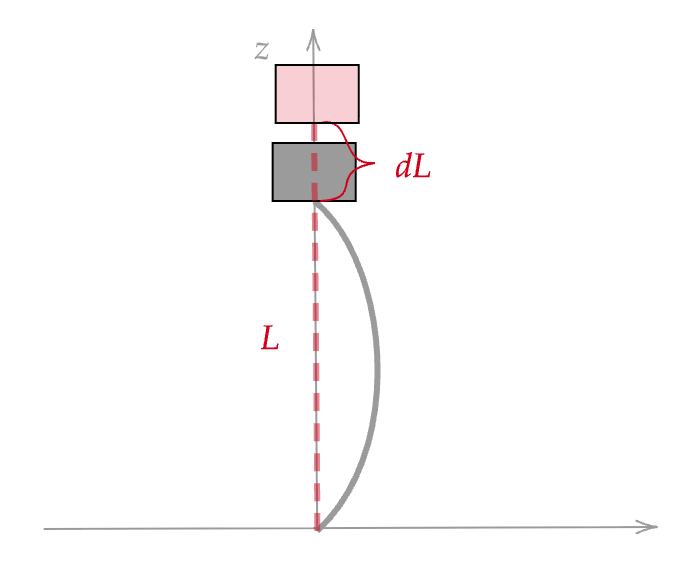
\includegraphics[width=0.7\linewidth]{files/euler_problem-85a6acb1fc4f4cee1ea1426b81e9491a.png}
\end{figure}